\documentclass[tikz]{standalone}

\usepackage{tikz}
\usetikzlibrary{positioning,shapes,backgrounds}
\usepackage{tkz-euclide}

\begin{document}

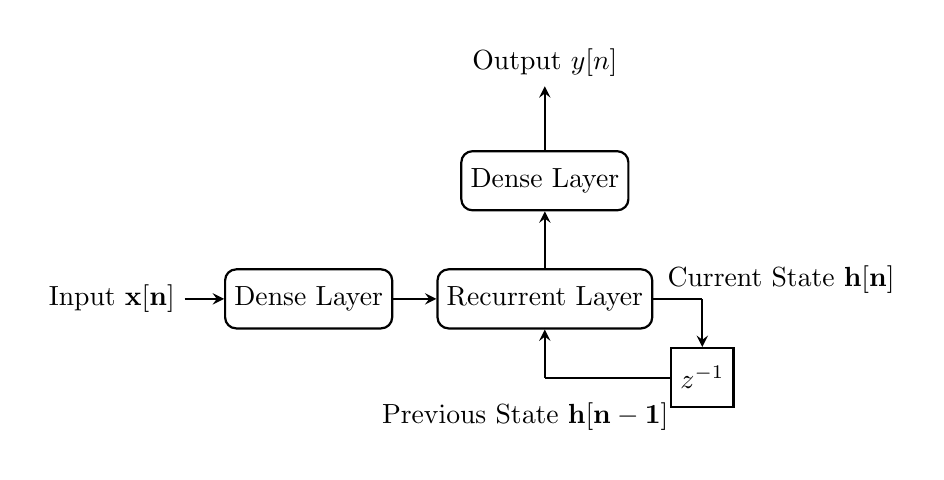
\begin{tikzpicture}[node distance=1.5cm, background rectangle/.style={fill=white}, show background rectangle]
    \tikzset{
        mynode/.style = {rectangle, rounded corners, line width=0.8pt, minimum width=1.0cm, minimum height=0.75cm, text centered, draw=black, fill=white},
        amp/.style = {regular polygon, regular polygon sides=3, draw, fill=white, text width=1em,
                      inner sep=1mm, outer sep=0mm, shape border rotate=-90, line width=0.8pt},
        arrow/.style = {thick,->,>=stealth},
        delay/.style = {rectangle, draw=black, line width=0.8pt, minimum height=0.75cm}
    }
    \node (input) {Input $\mathbf{x[n]}$};
    \node (dlayer) [mynode, right of=input, xshift=1.0cm] {Dense Layer};
    \node (rlayer) [mynode, right of=dlayer, xshift=1.5cm] {Recurrent Layer};
    \coordinate[right of=rlayer, xshift=0.5cm] (h0) ;
    \node (h0Label) [right of=h0, yshift=0.25cm, xshift=-0.5cm] {Current State $\mathbf{h[n]}$};
    \node (z1) [delay, below of=h0, yshift=0.5cm] {$z^{-1}$};
    \coordinate[below of=rlayer, yshift=0.5cm] (h1);
    \node (h1Label) [below of=h1, yshift=1.0cm, xshift=-0.25cm] {Previous State $\mathbf{h[n-1]}$};

    \draw [arrow] (input) -- (dlayer);
    \draw [arrow] (dlayer) -- (rlayer);
    \draw [thick] (rlayer) -- (h0);
    \draw [arrow] (h0) -- (z1);
    \draw [thick] (z1) -- (h1);
    \draw [arrow] (h1) -- (rlayer);

    \node (dense) [mynode, above of=rlayer] {Dense Layer};
    \node (out) [above of=dense] {Output $y[n]$};
    \draw [arrow] (rlayer) -- (dense);
    \draw [arrow] (dense) -- (out);
\end{tikzpicture}

\end{document}
